\chapter{Lower Energy Is Not Enough: Entropy and Free Energy}

\begin{kaichang}
Someone sprains an ankle in PE, and the teacher takes a flat instant cold pack from the first-aid kit. One squeeze makes a small pop. Seconds later the whole pouch is icy, chilling the ankle.

Play detective. Cooling means the process inside \textbf{absorbs heat}, taking it from hands and air. Yet nobody heats, ignites, or powers it; it happens by itself. Ice on the desk likewise melts at room temperature, absorbing heat spontaneously.

Strange: Chapter 27 just established a preference for lower energy, giving exothermic change its driving force. Ice and cold packs go the other way. Was the rule wrong, or incomplete? Guess the identity of another judge if falling energy is not enough.
\end{kaichang}

\section{The Broken Energy Rule}

Start with observations. A cold pack contains solid ammonium nitrate, \chem{NH_4NO_3}, and a water pouch. Breaking it starts dissolution, taking about \ud{26}{kJ} from surroundings per \ud{1}{mol} dissolved. Thus it cools. In Chapter 27's language, $\Delta H>0$ and the system loses on its energy account. The old preference for lower energy would forbid spontaneous change. Yet it proceeds and cannot be stopped once started, unless frozen in a refrigerator for a long time.

Such rule-breakers abound:

\begin{itemize}[itemsep=2pt]
\item Ice melts in a $25\,^{\circ}\mathrm{C}$ room: endothermic and spontaneous.
\item Open perfume spreads throughout a room without shaking or blowing; gas molecules disperse from a cluster into a large space without a driving energy decrease.
\item Sugar in hot water eventually sweetens the whole cup even without stirring.
\item Opening a carbonated drink sends dissolved \chem{CO_2} rushing out, despite heat absorption during escape.
\end{itemize}

Some processes obey: hot water cools as concentrated thermal energy spreads through the room. But the rule-breakers tell us enthalpy, $\Delta H$, is only one judge. Nature keeps another ledger.

\begin{shiyan}
\textbf{Take the Measure of Spontaneous Heat Absorption.} Materials: a commercial instant cold pack containing ammonium nitrate and water, a room thermometer, a dry towel, and timer. Procedure: (1) Record room temperature and feel the pack with the back of your hand. (2) Squeeze its inner pouch through the towel, shake gently for ten seconds, and start timing. (3) Every 30 seconds, feel the outside, preferably reading a thermometer held against it; note the minimum and recovery. (4) Watch whether ice forms outside: this is the key question. Safety note: \textbf{never open the outer pouch}, taste its contents, or squeeze them onto skin. Wrap and discard it afterward; sensitive skin should always use the towel. What to observe: it proceeds spontaneously, absorbs heat spontaneously, yet never freezes. Remember these three contrasts and explain them at the end. Without a pack, observe ice melting in a cup at room temperature, record temperatures, and ask why heat absorption needs no human help.
\end{shiyan}

\section{Why Particles ``Like'' to Spread}

Return to particles for the second ledger. Why does scent spread? Molecules have neither feet nor wishes, so why insist on dispersal?

They insist on nothing; probability suffices. Divide a box into halves, put four gas molecules left and vacuum right, then remove the partition. Each molecule has equal chances left or right, like a coin toss. All four on the left have only one arrangement, while two on each side have six. Count the possible left-hand pairs: AB, AC, AD, BC, BD, CD. More molecules make the disparity astonishing:

\begin{qiaoliang}
Put $N$ molecules in a two-sided box, each independently choosing a side. All $N$ on the same side give one arrangement out of $2^N$, a probability $1/2^N$.

For $N=4$, $1/16$ occurs occasionally. For $N=100$, roughly $1/10^{30}$ means even one observation per second since the Big Bang, about $4\times10^{17}$ seconds, would not catch it once. Your room holds about $10^{27}$ molecules, whose chance of all crowding back into half is $1/2^{10^{27}}$, too small even to write out.

Uniform dispersal is therefore no molecular goal; it corresponds to \textbf{overwhelmingly more arrangements}. It is not one special state but a name for unimaginably many nearly indistinguishable states.
\end{qiaoliang}

\begin{center}
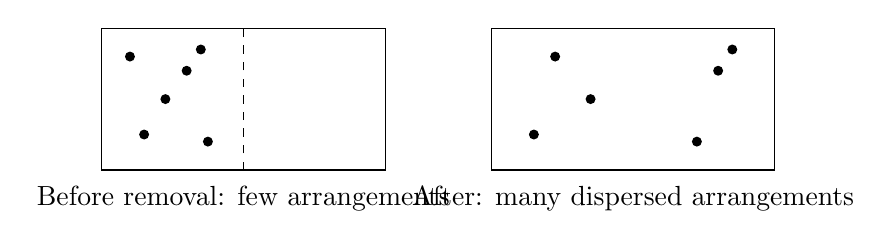
\begin{tikzpicture}[scale=0.9]
\draw (0,0) rectangle (4,2);
\draw[dashed] (2,0) -- (2,2);
\fill (0.6,0.5) circle (2pt); \fill (1.2,1.4) circle (2pt);
\fill (0.9,1.0) circle (2pt); \fill (1.5,0.4) circle (2pt);
\fill (0.4,1.6) circle (2pt); \fill (1.4,1.7) circle (2pt);
\node at (2,-0.4) {Before removal: few arrangements};
\draw (5.5,0) rectangle (9.5,2);
\fill (6.1,0.5) circle (2pt); \fill (8.7,1.4) circle (2pt);
\fill (6.9,1.0) circle (2pt); \fill (8.4,0.4) circle (2pt);
\fill (6.4,1.6) circle (2pt); \fill (8.9,1.7) circle (2pt);
\node at (7.5,-0.4) {After: many dispersed arrangements};
\end{tikzpicture}
\end{center}

(A representation: dot sizes are not real molecular sizes, and molecules never remain still.)

Energy plays the same game. Hot-water molecules carry concentrated thermal energy and room-air molecules less. Through collisions, energy has countless ways to spread evenly but few to concentrate further. Heat thus flows hot to cold not because mechanics bans the reverse, but because its probability is effectively zero.

Dispersal has three faces: particles spread in \textbf{space}, as scent diffuses; energy spreads \textbf{among particles}, as water cools; different particles \textbf{mix}, as sugar dissolves or saltwater joins pure water. All increase available arrangements. This perspective is the second law of thermodynamics: isolated systems tend toward greater entropy because many overwhelms few. Have you ever shaken mixed salt and pepper back apart, or seen cold coffee heat itself while freezing its table? Such reversed scenes violate no mechanical law, but never happen because countless particles would have to converge on extremely rare arrangements.

Now name the second account. More microscopic arrangements underlying a macroscopic state mean higher \textbf{entropy}. It counts ways of spreading: more dispersed particles and more evenly spread energy offer more arrangements and higher entropy.

\section{Entropy: Counting the Ways to Spread}

Give the intuition symbols: entropy is $S$, its change $\Delta S$. Because arrangements depend on particle number and energy, its unit is energy per temperature, $\mathrm{J/K}$, joules per kelvin. Counting sounds abstract, but useful consequences follow immediately:

\begin{itemize}[itemsep=2pt]
\item For the same substance, \textbf{gas entropy greatly exceeds liquid, which exceeds solid}. Gas explores a whole container with astronomical possibilities; crystal particles (Chapter 24) merely vibrate at fixed positions.
\item Higher temperature spreads particle energy more widely and increases entropy.
\item Thus melting ($\Delta S>0$), vaporization ($\Delta S\gg 0$), solid dissolution, and reactions producing more gas molecules increase entropy. Freezing, condensation, and crystallization decrease system entropy.
\end{itemize}

Mind the wording: entropy is \textbf{the number of microscopic arrangements}, not messiness. A crystal's entropy is low because fixed positions allow few choices, not because its lattice looks tidy. Disorder is an everyday association, not a definition. Count rather than judge neatness, and the later accounts will work.

Two examples help. Bubbling soda releases \chem{CO_2} from watery surroundings into vast space, giving $\Delta S>0$ and an entropy gain despite some heat absorption. Heating gas raises average kinetic energy and available energy levels, increasing arrangements and entropy. Covering hot soup, conversely, does not change its entropy itself, but blocks routes for dispersing it into surroundings. This links entropy increase with irreversible diffusion, heat transfer, and mixing.

\begin{wuqu}
``Entropy means disorder; an untidied room gains entropy.'' Half-right metaphors can mislead. Shake a supersaturated sodium acetate solution like that in warmers and neat needle crystals fill the cup spontaneously. Particles become highly ordered, yet the process proceeds because released heat raises surroundings' entropy more than crystallization lowers the system's. \textbf{System plus surroundings still gain entropy}. Life likewise assembles scattered molecules into ordered cells while exporting entropy through respiration and heat. Counting only system neatness leads to absurd claims that life or crystallization violates thermodynamics.
\end{wuqu}

\section{The Surroundings Have a Vote: Free Energy}

Now solve the case. Ammonium nitrate dissolving absorbs heat, $\Delta H>0$, losing on energy, but frees lattice ions to wander hydrated through water (Chapter 25), gaining entropy, $\Delta S>0$. Which account wins?

Nineteenth-century physicists found that constant temperature and pressure, everyday conditions, let the accounts combine. System heat goes to surroundings, increasing their entropy; the same heat has a larger entropy effect when surroundings are colder. A cold environment is initially quieter, so added heat matters more; a hot one barely notices. Surroundings' entropy change is therefore $-\Delta H/T$, added to the system's $\Delta S$. Positive total permits spontaneity. Rearranged as a system quantity, this becomes the American physicist Gibbs's \textbf{Gibbs free energy}, $G$:

\[\Delta G = \Delta H - T\Delta S\]

Read it simply: $\Delta G<0$ means spontaneous at constant temperature and pressure; $\Delta G>0$ favors the reverse; $\Delta G=0$ means equilibrium. The old enthalpy judge favors lower energy; the new $T\Delta S$ judge favors more arrangements. Temperature $T$ is their exchange rate: higher temperature increases entropy's value. Four combinations make this clear:

\begin{table}[h]
\centering
\begin{tabular}{cccl}
\toprule
$\Delta H$ & $\Delta S$ & $\Delta G$ & Result and example \\
\midrule
Negative (exothermic) & Positive (entropy rises) & Always negative & Always spontaneous, e.g. burning \\
Positive (endothermic) & Positive (entropy rises) & Negative when hot & Hotter favors it: cold packs, calcination \\
Negative (exothermic) & Negative (entropy falls) & Negative when cold & Colder favors it: freezing water \\
Positive (endothermic) & Negative (entropy falls) & Always positive & Never spontaneous \\
\bottomrule
\end{tabular}
\end{table}

The middle rows explain our title: \textbf{lower energy is not enough}. Endothermic processes with sufficient entropy gain at high enough temperature still have negative $\Delta G$: cold packs, melting ice, and bubbling soda. Freezing releases heat and proceeds in winter but not summer, because higher $T$ changes the balance of $-T\Delta S$. Thus \textbf{temperature can reverse a process's direction}. At $0\,^{\circ}\mathrm{C}$ water and ice tie with $\Delta G=0$; above, entropy wins and ice melts; below, enthalpy wins and water freezes.

Industry masters this principle. Limestone calcination, \[\chem{CaCO_3} \rightarrow \chem{CaO} + \chem{CO_2}\] absorbs heat but releases gas, greatly increasing entropy. Above about $900\,^{\circ}\mathrm{C}$, $T\Delta S$ exceeds $\Delta H$, giving negative $\Delta G$ and continuous quicklime production. Buildings have lime and cement because workers raise temperature past entropy's winning threshold; cooling immediately reverses the direction. The same equation explains why heating sometimes makes reactions reluctant: hot steam resists condensation.

Try real numbers for ice. Melting \ud{1}{mol}, a small spoonful of \ud{18}{g}, absorbs about \ud{6.0}{kJ}, reducing surroundings' entropy by $6000/T$. Escaping the lattice increases system entropy by about $6000/273\approx\ud{22}{J/K}$, estimated at melting. In a $25\,^{\circ}\mathrm{C}$ room, $T=298$ K, surroundings lose $-6000/298\approx-\ud{20}{J/K}$, so total $22-20=+\ud{2}{J/K}$ favors melting. At $-10\,^{\circ}\mathrm{C}$, $T=263$ K, surroundings give $-6000/263\approx-\ud{23}{J/K}$, so total $22-23=-\ud{1}{J/K}$ opposes melting and favors freezing. The dividing temperature is $T=273$ K, or $0\,^{\circ}\mathrm{C}$, where the total is zero. Childhood's rule that ice melts above zero is an arithmetic problem.

For any process, follow three steps: ask the enthalpy account, whether more bonds form or break and the sign of $\Delta H$; ask whether particles gain freedom through gas production, dissolution, or warming, and the sign of $\Delta S$; then use temperature to combine them into $\Delta G$. Direction emerges. Speed and whether a push is needed remain outside this checklist.

\section{Spontaneous Does Not Mean Fast}

Do not confuse $\Delta G<0$ with immediate action. Three facts:

\begin{itemize}[itemsep=2pt]
\item Diamond in a ring, if you have one, has $\Delta G<0$ for becoming graphite at ordinary conditions. Yet it stays unchanged for hundreds of millions of years; jewelers lose no sleep.
\item Rusting iron clearly has negative $\Delta G$, yet corrosion through a nail takes years. Explosive oxidation can take a millionth of a second.
\item Hydrogen and oxygen in one bottle have strongly negative $\Delta G$ for water formation, yet coexist peacefully for a year until a spark arrives.
\end{itemize}

Distinguish \textbf{which direction} from \textbf{how fast}. $\Delta G$ answers only the first, locating the finish line without describing intervening hills. Diamond-to-graphite is favorable, but each carbon must escape three strong covalent bonds (Chapter 24) to rearrange. The enormous barrier is inaccessible to almost all room-temperature atoms, stalling spontaneity for eons.

Negative $\Delta G$ likewise gives wildly different schedules: seconds for cold packs, minutes for iron-oxidation warmers, years for railings to rust through, tens of thousands of years for rock weathering. Identical directional verdicts have unrelated timetables, set by another authority.

Remember both: spontaneous means neither fast nor trigger-free. A spark does not supply hydrogen--oxygen combustion's driving energy, which exceeds the spark by tens of thousands of times. It helps the first molecules cross the barrier, and their heat pushes later molecules onward. Firecrackers, gas stoves, and engines all use a key to unlock an already favorable route. Direction and speed have separate ledgers; activation energy governs the latter in Chapter 29.

\begin{zhengju}
Entropy as arrangement counting once provoked a career-defining controversy. In the 1870s, Boltzmann argued that thermal laws reduce to atomic statistics. He showed isolated entropy increasing or remaining constant, not because a mechanical decree forbids decreases, but because decreasing arrangements are overwhelmingly rare. He condensed the answer into $S=k\ln W$: entropy equals a constant times the logarithm of arrangement count $W$.

Nobody had seen atoms. Authorities led by Mach viewed them as convenient fictions and atomic thermodynamics as risky metaphysics. Boltzmann repeatedly defended himself in papers and lectures against opponents denying molecules. A subtler objection concerned time: reversible molecular laws allow reversed collision films without mechanical violations, so why does the visible world have direction? His answer, probability rather than mechanics, outran contemporary acceptance.

Boltzmann died in depression in 1906 before final vindication. Evidence arrived almost simultaneously: Einstein's 1905 Brownian-motion account calculated molecular impacts behind Chapter 25's dancing pollen, and Perrin's microscopic experiments confirmed it. Atoms existed and statistical explanation prevailed. Today $S=k\ln W$ marks Boltzmann's grave. Remember not victory or defeat but method: testable predictions, such as precise Brownian statistics, ultimately let experiments judge philosophical objections.
\end{zhengju}

\section{The Ledger's Fine Print}

$\Delta G$ is useful, with conditions printed in its manual:

\begin{itemize}[itemsep=2pt]
\item \textbf{Direction only at constant temperature and pressure}. Deep space, Earth's core, and high-pressure vessels may require recalculation or other free energies.
\item \textbf{Direction, not rate}. Negative $\Delta G$ may be immeasurably slow; speeding it requires activation-energy and catalyst studies (Chapters 29 and 30).
\item \textbf{Possibility, not motion}. Negative $\Delta G$ can stall en route, while $\Delta G=0$ is not stillness but balanced forward and reverse activity (Chapter 31).
\item \textbf{The entropy law applies to isolated systems}. Your room, body, and Earth are not isolated. Earth receives low-entropy sunlight and emits high-entropy thermal radiation. Local decreases from freezing, growth, or city-building are legitimate if larger increases occur elsewhere. Using entropy to ban ordered structures misapplies the law's scope.
\end{itemize}

\section{Back to the Cold Pack}

Return to the first-aid kit with complete accounts. Dissolving ammonium nitrate breaks lattice attractions and builds hydration shells, net endothermic with $\Delta H>0$, drawing the deficit from your skin. But freed hydrated ions greatly increase $\Delta S$. Room-temperature $T$ makes that gain outweigh enthalpy's cost, producing $\Delta G<0$ and dissolution until rising concentration balances the books.

The experiment's contrasts now align. It is \textbf{spontaneous} because $\Delta G<0$ needs no push. It \textbf{spontaneously absorbs heat} because entropy wins, increasingly strongly at higher temperature. Its \textbf{outside never freezes} because finite heat absorption lowers temperature only a dozen or so degrees, still far above $0\,^{\circ}\mathrm{C}$. Even below zero, ion-filled water freezes less readily than pure water, as Chapter 25's challenge calculated.

Three easily confused statements become clear: spontaneous yet \textbf{not exothermic}, since enthalpy is not alone; spontaneous yet \textbf{finite}, as concentration moves $\Delta G$ toward zero; spontaneous and incidentally fast, though speed is luck, not a gift of spontaneity. Diamond lacks that luck.

\section{After Direction Comes Speed}

We have issued reactions their directional permits: enthalpy and entropy combine through temperature into $\Delta G$, whose sign decides direction and can be reversed by heating. Metallurgists use it to find iron-extraction temperatures, chemical engineers to judge worthwhile reactions, and doctors in freeze-drying vaccines and plasma. Lower temperature and pressure redirect melting so water leaves directly as vapor without decay or heat damage.

Yet direction is only half the story. Diamond delays graphite formation for eons; explosives and rust differ in rate by over a dozen orders of magnitude; summer food spoils overnight while refrigeration preserves it another week. Thermodynamics governs direction, another set of rules speed: how hard particles must collide and how high a barrier they must cross to change. Chapter 29 measures that barrier.

\begin{tiaozhan}
Calculate Boltzmann's account yourself. In $S=k\ln W$, $W$ counts microstates and $k=\ud{1.38\times10^{-23}}{J/K}$. Let \ud{1}{mol} gas, $6.02\times10^{23}$ molecules, expand from half a box to all of it. Each doubles its possible positions, multiplying $W$ by $2^{6.02\times10^{23}}$:
\[\Delta S = k\ln\left(2^{6.02\times10^{23}}\right) = k\times 6.02\times10^{23}\times\ln 2 \approx 8.31\times 0.693 \approx \ud{5.8}{J/K}\]
Notice $8.31$, the molar gas constant $R$ familiar from Chapter 26. Macroscopic $R$ and microscopic $k$ are linked by a \ud{6.02\times10^{23}}{} bridge, statistical mechanics' beautiful view of counting behind constants. Optional though it is, understanding this lets you feel the meaning of the formula on Boltzmann's grave.
\end{tiaozhan}

\section*{Try It}

\begin{sikaoti}
\item Draw a cold pack before dissolution, with ordered ammonium nitrate and separate water, and after, with dispersed hydrated ions. Mark heat flow and entropy changes in system and surroundings, noting that this is a representation, not actual appearance.
\item Without formulas, explain through arrangement counts why red ink disperses in water but never spontaneously regathers into one drop. Would a reversed video violate a mechanical law?
\item Freezing releases heat, $\Delta H<0$, and reduces entropy, $\Delta S<0$. Use $\Delta G=\Delta H-T\Delta S$ to explain freezing at $-18\,^{\circ}\mathrm{C}$ but never at $10\,^{\circ}\mathrm{C}$. What condition defines the temperature where ice and water tie?
\item Classify system entropy increase or decrease, explaining each: perfume evaporating, vapor fogging a mirror, heated baking soda releasing \chem{CO_2}, and plants assembling \chem{CO_2} and water into glucose.
\item Where is the error in ``paper is combustible with $\Delta G<0$, so this book might ignite itself anytime''? Separate direction from speed and name the barrier preventing it, next chapter's protagonist.
\item Look up limestone calcination temperature and explain to family why kilns must become so hot rather than simply waiting for room-temperature reaction, using endothermic entropy-increasing reactions favored by heat.
\end{sikaoti}
